\section{Descripción arquitectónica}

Ahora bien, en cuanto a la arquitectura del sistema implementado en Verilog HDL, se tiene que la PCS consiste de 5 módulos: \texttt{TRANSMIT}, \texttt{RECEIVE}, \texttt{SYNCHRONIZATION}, \texttt{CARRIER-SENSE} y \texttt{AUTO-NEGOTIATION} \cite{IEEE8023-2018}.
Según los alcances establecidos en el enunciado del proyecto, se implementaron únicamente los tres primeros y se aseguró de que las señales manejadas por los otros módulos tuvieran el comportamiento esperado.

Entonces, a continuación se explican cada uno de los módulos, las señales de entrada y salida que los conforman, los estados seleccionados y el diagrama ASM que describe el comportamiento de la máquina de estados.

\subsection{Módulo \texttt{TRANSMIT}}

Respecto al submódulo de transmisión, este está dividido en dos máquinas de estado separadas: \textit{transmit code-group} y \textit{transmit ordered set}.
En la Figura \ref{fig:transmisor-diagrama_bloques}, se muestra un diagrama de bloques donde se indican las conexiones de las máquinas de estados.

\begin{figure}[htb]
    \centering
    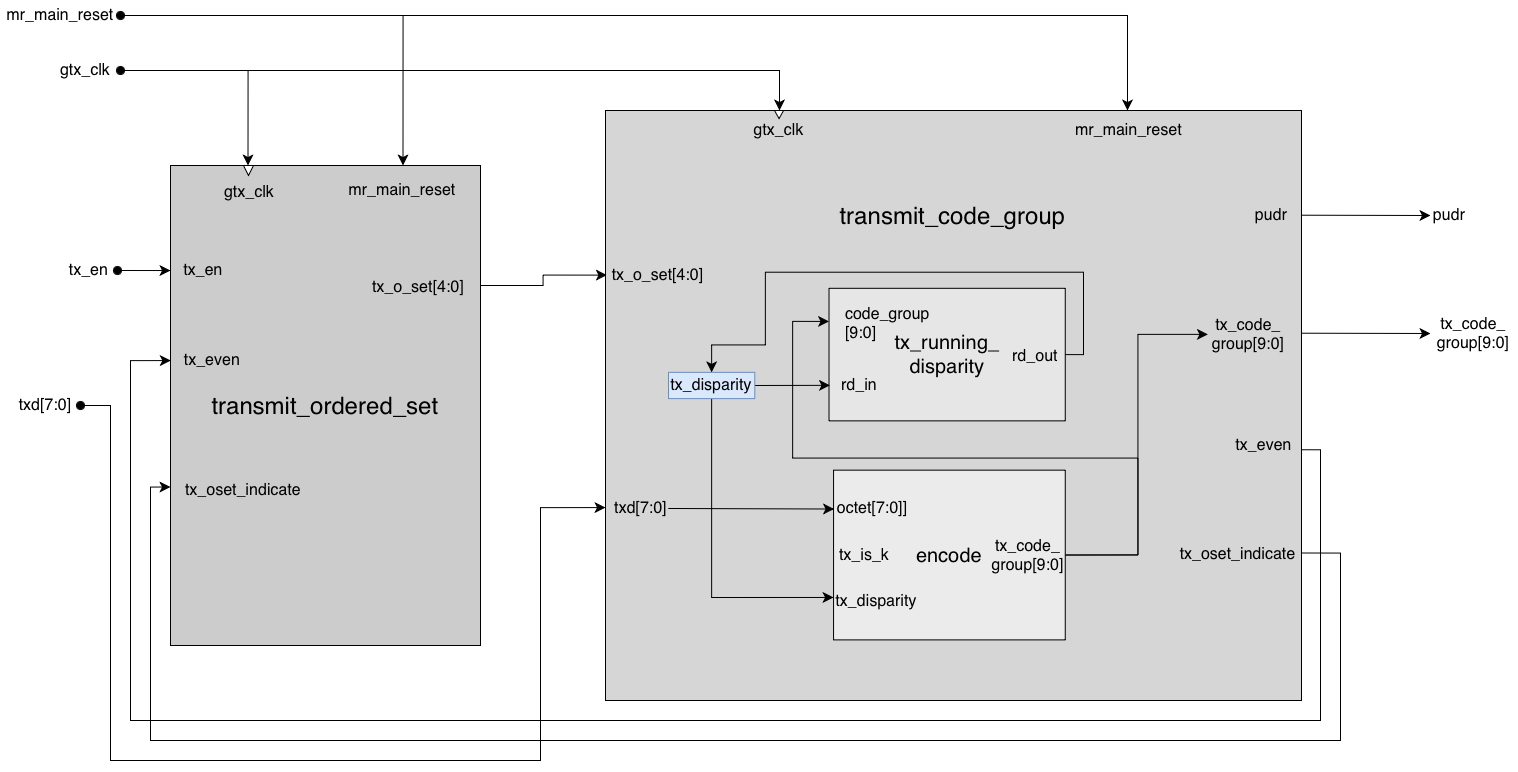
\includegraphics[width=\textwidth]{images/diagrama-bloques-transmisor.png}
    \caption{Diagrama de bloques del módulo \texttt{TRANSMIT}.}
    \label{fig:transmisor-diagrama_bloques}
\end{figure}

Antes de continuar con la explicación de las máquinas de estado principales, se van a explicar los bloques combinacionales \texttt{encode} y \texttt{running\_disparity} creados para facilitar el diseño.
El primero corresponde a un \textit{lookup table} que recibe el \texttt{running\_disparity} actual y la señal \texttt{txd} de 8 bits.
A partir de estos datos, coloca en su salida el \textit{code-group} resultante de 10 bits.

El segundo corresponde al módulo que recibe el \textit{code-group} actual junto con el \texttt{running\_disparity} actual y calcula el siguiente \texttt{running\_disparity}.
Por lo tanto, ambos módulos funcionan para modularizar el código de la máquina de estados \texttt{transmit\_code\_group} y facilita el diseño y mantenimiento del código.

Ahora sí, se continúa con la explicación de la arquitectura de las máquinas de estados principales.

\subsubsection{Submódulo \texttt{transmit\_code\_group}}

Inicialmente, se realiza una descripción del funcionamiento esperado de este bloque.
El módulo selecciona el octeto apropiado para transmisión, ya sea datos o alguno de los símbolos especiales \texttt{/S/}, \texttt{/T/}, \texttt{/R/} o \texttt{/I/}.
Además, determina si el símbolo corresponde a un carácter de tipo K mediante la señal \texttt{tx\_is\_k}, requerida para la codificación 8b/10b.
También actualiza la señal \texttt{tx\_even} con el fin de distinguir entre ciclos pares e impares.
Posteriormente, genera el code-group de 10 bits en \texttt{tx\_code\_group}.
Una vez que el code-group está listo, activa la señal \texttt{tx\_oset\_indicate} para informar al módulo \texttt{transmit\_ordered\_set}.
Finalmente, habilita la señal \texttt{pudr} cuando el code-group se encuentra disponible para ser enviado hacia la capa PMA.

En el estándar IEEE 802.3, se muestra un diagrama de estados complejo con estados repetidos y/o sobrantes, que no entran dentro del contexto del proyecto, ya sea por ser de manejo de errores o de configuración.
Estos fueron eliminados y los finales se muestran en la Figura \ref{fig:transmit_code_group_asm}.

\begin{figure}[htb]
    \centering
    
\includegraphics[width=0.8\textwidth]{images/transmit_code_group_asm.png}
    \caption{Diagrama ASM del módulo \texttt{transmit\_code\_group}.}
    \label{fig:transmit_code_group_asm}
\end{figure}

Para la codificación de los estados del diagrama ASM correspondiente, se utilizó \textit{one-hot encoding}.
Esta es fundamental para evitar condiciones de carrera en implementaciones reales.
Estos se muestran en el Cuadro \ref{tab:estados-transmit_code_group}.

\begin{table}[htb]
    \centering
    \begin{tabular}{cc}
    \hline
    \textbf{Estado} & \textbf{Codificación} \\
    \hline
    \texttt{GENERATE\_CODE\_GROUPS} & 2'b01 \\
    \texttt{IDLE\_2} & 2'b10 \\
    \hline
    \end{tabular}
    \caption{Estados del módulo \texttt{transmit\_code\_group}.}
    \label{tab:estados-transmit_code_group}
\end{table}

Para completar la descripción arquitectónica, en el Cuadro \ref{tab:transmit_code_group_senales}, se muestran las señales de entrada y salida del módulo \texttt{transmit\_code\_group}.
Así como una descripción del funcionamiento de la señal en cuestión.

\begin{table}[htb]
    \centering
    \begin{tabular}{lcp{7cm}}
    \hline
    \textbf{Señal} & \textbf{Tipo} & \textbf{Descripción} \\ \hline
    \texttt{gtx\_clk} & Entrada & Reloj de transmisión del bloque PCS. \\
    \texttt{mr\_main\_reset} & Entrada & Reinicio global del transmisor, activo en alto. \\
    \texttt{txd [OCTET\_WIDTH-1:0]} & Entrada & Octeto de datos a transmitir cuando \texttt{tx\_o\_set} indica \texttt{/D/}. \\
    \texttt{tx\_o\_set [TX\_O\_SET\_WIDTH-1:0]} & Entrada & Identificador del tipo de ordered set (\texttt{/I/}, \texttt{/S/}, \texttt{/D/}, \texttt{/T/}, \texttt{/R/}). \\
    \texttt{tx\_code\_group [CG\_WIDTH-1:0]} & Salida & Code-group que se envía hacia la capa PMA. \\
    \texttt{tx\_even} & Salida & Indicador de ciclo par/impar. \\
    \texttt{tx\_oset\_indicate} & Salida & Señal que indica que el code-group actual se encuentra listo para que \texttt{transmit\_ordered\_set} avance. \\
    \texttt{pudr} & Salida & Señal de indicación hacia la PMA de que existe un nuevo code-group disponible en \texttt{tx\_code\_group}. \\ \hline
    \end{tabular}
    \caption{Señales de entrada y salida de \texttt{transmit\_code\_group}.}
    \label{tab:transmit_code_group_senales}
\end{table}

\subsubsection{Submódulo \texttt{transmit\_ordered\_set}}

Respecto al módulo \texttt{transmit\_ordered\_set}, se tiene que este se encarga de generar el comportamiento descrito a continuación:
El módulo permanece en el estado \texttt{IDLE} (representado por \texttt{/I/}) cuando la transmisión no se encuentra habilitada.
Una vez que la señal \texttt{tx\_en} se activa, el módulo detecta el inicio de una trama y emite el símbolo \texttt{/S/} (\textit{Start of Packet}).
Posteriormente, transmite \texttt{/D/} mientras existan datos válidos disponibles.
Al finalizar la trama, genera el símbolo \texttt{/T/} y, según el valor de \texttt{tx\_even}, determina si es necesario aplicar \textit{carrier extend} mediante la emisión del símbolo \texttt{/R/}.

Adicionalmente, se muestra en la Figura \ref{fig:transmit_ordered_set_asm} el diagrama ASM simplificado del estándar IEEE 802.3, al igual que en el caso anterior.
Se simplificaron estados principalmente para coincidir con las temporaciones necesarias según los ciclos de reloj que debe tomar.
Para ello, se siguieron las indicaciones dadas por el profesor en clase.

\begin{figure}[htb]
    \centering
    
\includegraphics[width=0.45\textwidth]{images/transmit_ordered_set_asm.png}
    \caption{Diagrama ASM del módulo \texttt{transmit\_ordered\_set}.}
    \label{fig:transmit_ordered_set_asm}
\end{figure}

Los estados del diagrama ASM fueron codificados con \textit{one hot} y su código respectivo se muestra en el Cuadro \ref{tab:estados-transmit_ordered_set}.

\begin{table}[htb]
    \centering
    \begin{tabular}{cc}
    \hline
    \textbf{Estado} & \textbf{Codificación} \\
    \hline
    \texttt{XMIT\_DATA} & 3'b001 \\
    \texttt{TX\_PACKET} & 3'b010 \\
    \texttt{EPD} & 3'b100 \\
    \hline
    \end{tabular}
    \caption{Estados del módulo \texttt{transmit\_ordered\_set}.}
    \label{tab:estados-transmit_ordered_set}
\end{table}

Finalmente, las señales de entrada y salida de este submódulo, se indican en el Cuadro \ref{tab:transmit_ordered_set_senales}.
Adicionalmente, se agregó una breve descripción de lo que significan.

\begin{table}[H]
    \centering
    \begin{tabular}{lcp{7cm}}
    \hline
    \textbf{Señal} & \textbf{Tipo} & \textbf{Descripción} \\ 
    \hline
    \texttt{gtx\_clk} & Entrada & Reloj de transmisión del bloque PCS. \\
    \texttt{mr\_main\_reset} & Entrada & Reinicio global del transmisor, activo en alto. \\
    \texttt{tx\_even} & Entrada & Indicador de ciclo par/impar para decidir la aplicación de \textit{carrier extend}. \\
    \texttt{tx\_oset\_indicate} & Entrada & Señal que indica que el \textit{code group} actual ya se envió. \\
    \texttt{tx\_en} & Entrada & Habilitación de transmisión. \\
    \texttt{tx\_o\_set [TX\_O\_SET\_WIDTH-1:0]} & Salida & Identificador del ordered set a enviar (\texttt{/I/}, \texttt{/S/}, \texttt{/D/}, \texttt{/T/}, \texttt{/R/}). \\ \hline
    \end{tabular}
    \caption{Señales de entrada y salida de \texttt{transmit\_ordered\_set}.}
    \label{tab:transmit_ordered_set_senales}
\end{table}

\subsection{Módulo \texttt{SYNCHRONIZATION}}

En la Figura \ref{sincBlock} se muestra el diagrama de bloques estipulado para el módulo de \texttt{SYNCHRONIZATION}, con sus respectivas entradas y salidas.
El principal punto a destacar es la salida del \texttt{SUDI}, la cual en este caso es de 11 bits, donde los primeros 10 bits corresponden al code-group proveniente del \texttt{PUDI} y el último es el correspondiente a \texttt{rx\_even}.

\begin{figure}[H]
    \centering
    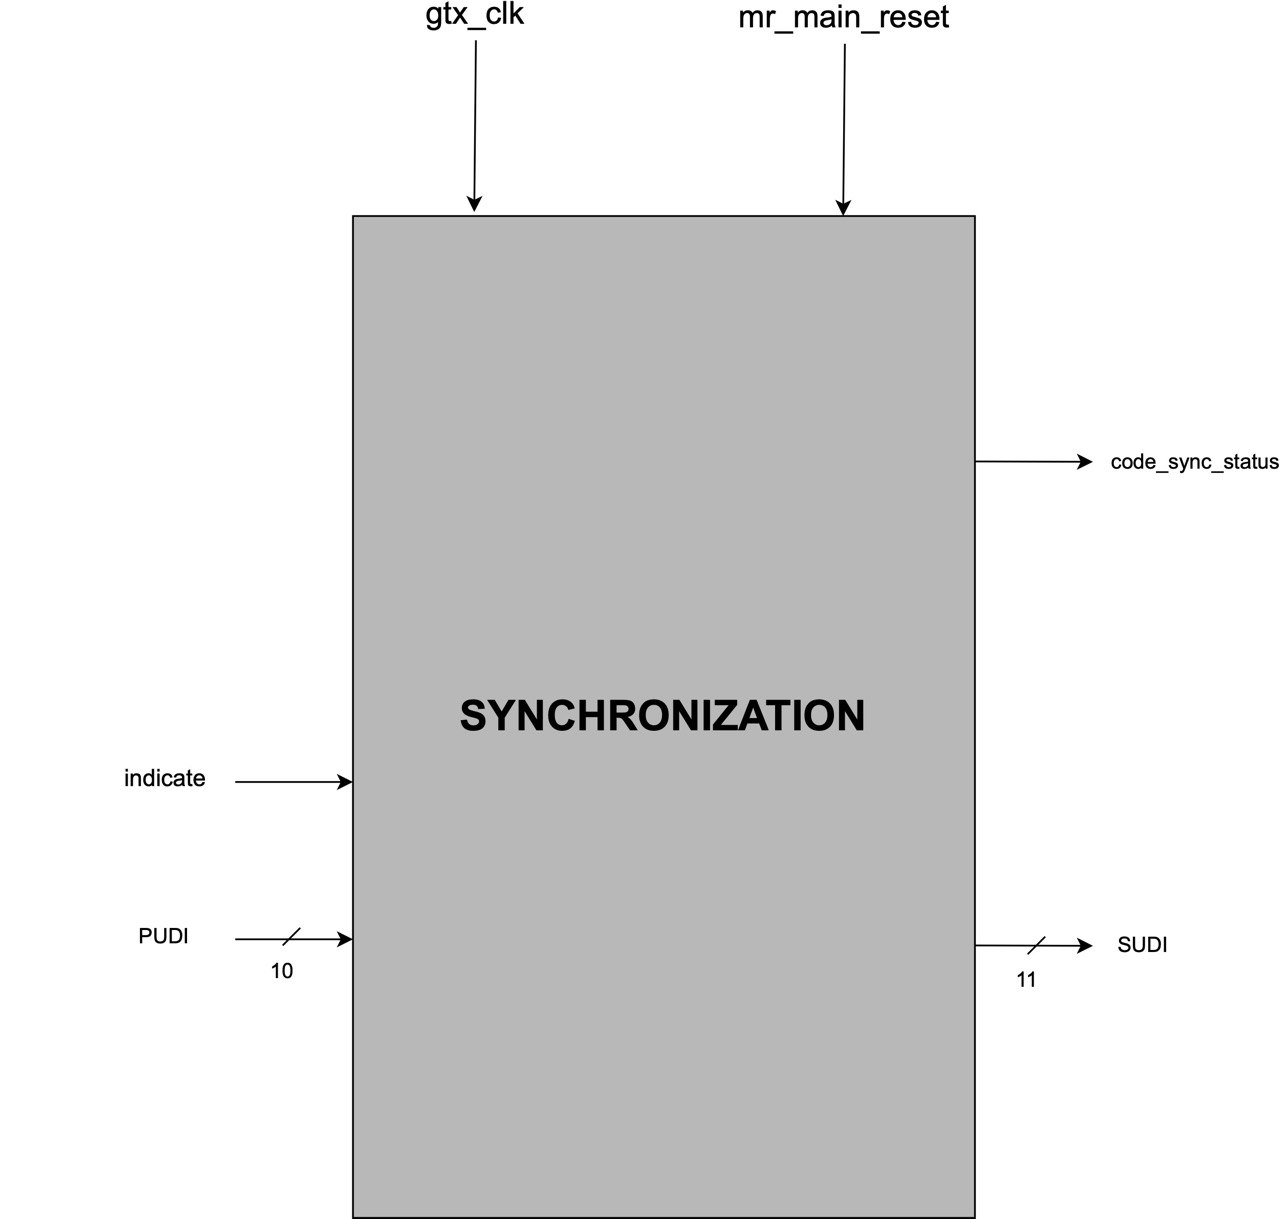
\includegraphics[width=0.6\textwidth]{images/sync_block.jpg}
    \caption{Diagrama de bloques del módulo \texttt{Synchronization}.}
    \label{sincBlock}
\end{figure}

Asimismo, dentro de este módulo, se tiene una instancia de \texttt{pudi\_checker}, que corresponde a un submódulo combinacional, que permite clasificar los \texttt{PUDI} recibidos en válidos/inválidos.

Para la sincronización inicial a partir del estado \texttt{LOSS\_OF\_SYNC}, se utilizaron contadores para ahorrar estados en este proceso.
Para el proceso de pérdida de sincronización, se mantuvo la estructura de estados mostrada en el estándar IEEE 802.3, con el fin de simplificar la programación, entendimiento y estructura del código.

En el Cuadro \ref{entradasysalidasSync} se observa con más detalle las entradas y salidas del módulo de \texttt{SYNCHRONIZATION}. 
Además, en el Cuadro \ref{estadosSync} se muestran los estados referentes al presente módulo, junto con una breve descripción de lo que hace cada uno. 

\begin{table}[htb]
\centering
\begin{tabular}{lcp{7cm}}
\hline
\textbf{Señal} & \textbf{Tipo} & \textbf{Descripción} \\ \hline
\texttt{mr\_main\_reset} & Entrada &   Reset activo en alto. Inicializa el sistema y fuerza el estado IDLE. \\
\texttt{clk} & Entrada & Señal de reloj principal del sistema. \\
\texttt{indicate} & Entrada & Indica que hay un code-group recibido. Proviene de la señal PUDR del transmisor (en \textit{loopback}). \\
\texttt{PUDI[CG\_WIDTH-1:0]} & Entrada & Code-group recibido desde el PMA. \\
\texttt{code\_sync\_status} & Salida & Indica sincronización adquirida. \\
\texttt{SUDI[CG\_WIDTH:0]} & Salida &  Code-group extendido a 11 bits (PUDI + rx\_even). \\ \hline
\end{tabular}
\caption{Señales de entrada y salida del módulo \texttt{SYNCHRONIZATION}.}
\label{entradasysalidasSync}
\end{table}

\begin{table}[H]
    \centering
    \begin{tabular}{ccp{7cm}}
    \hline
    \textbf{Estado} & \textbf{Código} & \textbf{Descripción} \\ \hline
    \texttt{LOSS\_OF\_SYNC} & 10'b0000000001 & Indica pérdida de sincronización. Se espera la aparición de una comma /K28.5/ válida. \\
    \texttt{COMMA\_DETECT} & 10'b0000000010 & Se detecta la comma por primera vez. Verifica que el siguiente code-group sea un D válido. \\
    \texttt{ACQUIRE\_SYNC} & 10'b0000000100 & Se detecta un dato válido, espera a que se lleguen a dos commas y dos datos para estar sincronizado. \\
    \texttt{SYNC\_ACQUIRED\_1} & 10'b0000001000 & Primer nivel de sincronización establecida. \texttt{rx\_even} alterna y se valida la calidad de los code-groups. \\
    \texttt{SYNC\_ACQUIRED\_2} & 10'b0000010000 & Un error detectado. Espera un code-group válido para volver a sincronizarse o uno inválido para seguir perdiendo sincronía. \\
    \texttt{SYNC\_ACQUIRED\_2A} & 10'b0010000000 & Se detectó un code-group válido después del primer inválido. Requiere 3 válidos para volver a estar sincronizado totalmente. \\
    \texttt{SYNC\_ACQUIRED\_3} & 10'b0000100000 & Dos code-groups inválidos. Mismo funcionamiento que \texttt{SYNC\_ACQUIRED\_2}. \\
    \texttt{SYNC\_ACQUIRED\_3A} & 10'b0100000000 & Mismo funcionamiento que \texttt{SYNC\_ACQUIRED\_2A}, pero para dos code-groups inválidos detectados. \\
    \texttt{SYNC\_ACQUIRED\_4} & 10'b0001000000 & Tres code-groups inválidos. \\
    \texttt{SYNC\_ACQUIRED\_4A} & 10'b1000000000 & Mismo funcionamiento que \texttt{SYNC\_ACQUIRED\_2A}, pero para tres code-groups inválidos. \\ \hline
    \end{tabular}
    \caption{Estados del módulo \texttt{SYNCHRONIZATION}.}
    \label{estadosSync}
\end{table}

Por último, se muestra el diagrama de estados ASM planteado para el módulo de \texttt{SYNCHRONIZATION} en la Figura \ref{asmSync}. 

\begin{figure}[H]
    \centering
    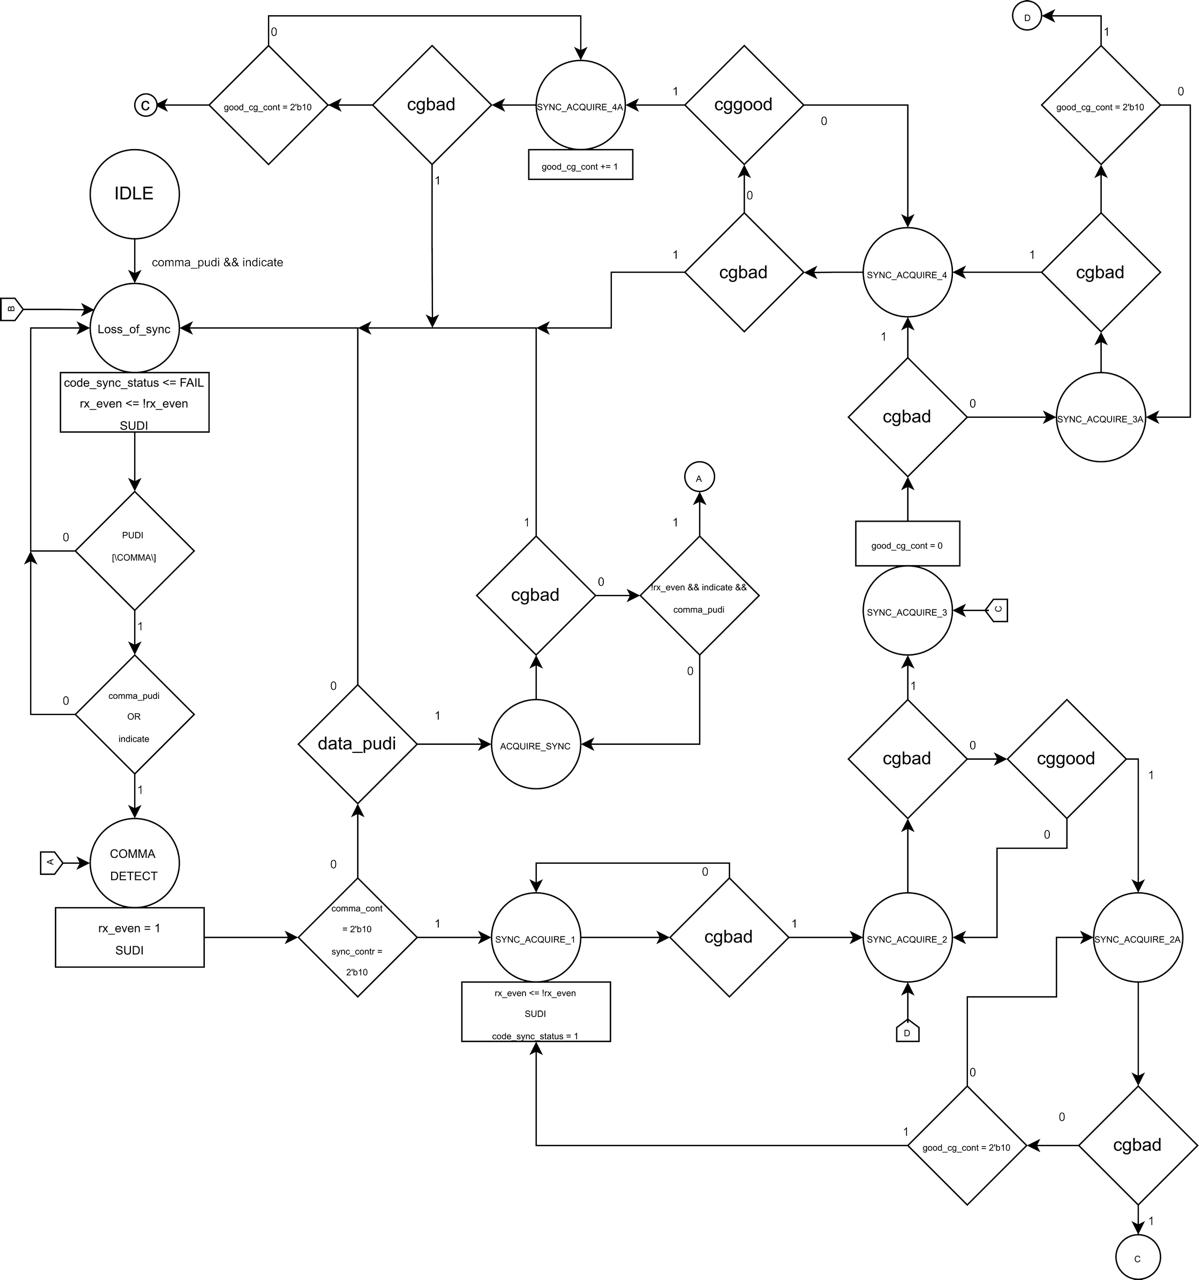
\includegraphics[width=\textwidth]{images/synchronization_ASM.jpg}
    \caption{Diagrama ASM del módulo \texttt{SYNCHRONIZATION}.}
    \label{asmSync}
\end{figure}


\subsection{Módulo \texttt{RECEIVE}}

Para el módulo de recepción, se trabajó instanciando 2 módulos, los cuales están dentro del módulo principal del receptor, tal y como se observa en la Figura \ref{receive_block}.
Se tiene un submódulo \texttt{running\_disparity}, el cual se encarga de calcular el próximo valor del running disparity según el running disparity actual y el \texttt{rx\_code\_group}.
Además, el módulo de \texttt{decode} se encarga de convertir de 10 bits a 8 bits el code-group recibido.
Este necesita el valor actual del running disparity y el \texttt{rx\_code\_group} para poder decodificar de manera correcta, y con esto se obtiene el valor del octeto y se envía a través de la salida \texttt{rxd}.

\begin{figure}[H]
    \centering
    
\includegraphics[width=\linewidth]{images/receive_block.png}
    \caption{Diagrama de bloques del módulo \texttt{RECEIVE}.}
    \label{receive_block}
\end{figure}

Las señales que están en el módulo de \texttt{RECEIVE} se observan en el Cuadro \ref{señales_receive}, donde se da una breve descripción de cada señal y su tipo.
\begin{table}[H]
    \centering
    \begin{tabular}{ccp{7cm}}
    \hline
    \textbf{Señal} & \textbf{Tipo} & \textbf{Descripción} \\
    \hline
    \texttt{rx\_clk} & Entrada & Reloj con el que funciona el receptor para el envio de datos. \\
    \texttt{mr\_main\_reset} & Entrada & Controla el reinicio de la PCS (activo en alto). \\
    \texttt{SUDI[10:0]} & Entrada & Señal enviada por el proceso de sincronización al proceso de recepción que contiene los bits del code-group y también el \texttt{rx\_even} (en el LSB). \\
    \texttt{sync\_status} & Entrada & Indica la sincronización (activo en alto). \\
    \texttt{rxd[7:0]} & Salida & Es el valor que entrega el receptor a la interfaz GMII. \\
    \texttt{rx\_dv} & Salida & Indica que los valores de \texttt{rxd} son válidos. \\
    \texttt{rx\_er} & Salida & Indica que los valores de \texttt{rxd} contienen un error. \\
    \hline
    \end{tabular}
    \caption{Señales del módulo \texttt{RECEIVE}.}
    \label{señales_receive}
\end{table}

\indent Además, se simplificaron los estados del módulo \texttt{RECEIVE}, pasando a tener 6 estados de 31 estados que contiene el estándar en el caso del receptor.
Además, para los estados implementados se utilizó la codificación \textit{one-hot}, estos se pueden observar en el Cuadro \ref{estados_receive}.

\begin{table}[H]
    \centering
    \begin{tabular}{cc}
    \hline
    \textbf{Estado} & \textbf{Codificación} \\
    \hline
    \texttt{LINK\_FAILED} & 6'b000001 \\
    \texttt{WAIT\_FOR\_K} & 6'b000010 \\
    \texttt{RX\_K} & 6'b000100 \\
    \texttt{IDLE\_D} & 6'b001000 \\
    \texttt{RECEIVE} & 6'b010000 \\
    \texttt{TRI\_RRI} & 6'b100000 \\
    \hline
    \end{tabular}
    \caption{Estados del módulo \texttt{RECEIVE}.}
    \label{estados_receive}
\end{table}

A continuación, en la Figura \ref{receive_asm} se presenta el diagrama ASM simplificado que se utilizó para el funcionamiento del módulo de \texttt{RECEIVE}.

\begin{figure}[H]
    \centering
    
\includegraphics[width=0.8\textwidth]{images/receive_asm.png}
    \caption{Diagrama ASM de la máquina de estados de \texttt{RECEIVE.}}
    \label{receive_asm}
\end{figure}
